% ADD/REMOVE THE 'answers' OPTION TO INCLUDE/SUPPRESS SOLUTIONS
\documentclass[11pt,addpoints]{exam}


\newcommand{\hwnum}{1}
\newcommand{\duedate}{January 15}

% in order to compile this file you will need to get 'header.tex'
% and make the line below point to the appropriate file path
\RequirePackage{microtype}
\RequirePackage{mathtools}
\RequirePackage{amsthm}
\RequirePackage{amssymb}
\RequirePackage{xspace}
\RequirePackage[shortlabels]{enumitem}
\RequirePackage{xcolor}
\RequirePackage{hyperref}
\RequirePackage[capitalize,nameinlink,noabbrev]{cleveref} % must load after hyperref
\usepackage{fvextra} % To use Verbatim
\RequirePackage[boxed]{algorithm}
\RequirePackage[noend]{algpseudocode}
\RequirePackage{tikz}

\hypersetup{breaklinks=true,
    colorlinks=true,
    linkcolor=blue,
    filecolor=blue,
    citecolor=blue,
    urlcolor=blue}

\algrenewcommand{\algorithmiccomment}[1]{\texttt{//} #1}
\algrenewcommand\algorithmicrequire{\textbf{Input:}}
\algrenewcommand\algorithmicensure{\textbf{Output:}}


% allow cleveref to label and reference enumerables defined in the exam class.
% these automatically define corresponding \Crefname as well.

% https://tex.stackexchange.com/questions/126020/cleveref-doesnt-use-correct-capitalized-name-if-used-with-amsthm
\makeatletter
\if@cref@capitalise
\crefname{question}{Question}{Questions}
\Crefname{partno}{Part}{Parts}
\crefname{subpart}{Subpart}{Subparts)}
\crefname{subsubpart}{Subsubpart}{Subsubparts}
\else
\crefname{question}{question}{questions}
\crefname{partno}{part}{parts}
\crefname{subpart}{subpart}{subparts}
\crefname{subsubpart}{subsubpart}{subsubparts}
\fi
\makeatother

% numeric sets in "blackboard" font

\newcommand{\N}{\mathbb{N}}
\newcommand{\Z}{\mathbb{Z}}
\newcommand{\R}{\mathbb{R}}
\newcommand{\Q}{\mathbb{Q}}
\newcommand{\C}{\mathbb{C}}
\newcommand{\Prop}{\mathbb{P}}

% paired delimiters

\DeclarePairedDelimiter\abs{\lvert}{\rvert}
\DeclarePairedDelimiter\length{\lVert}{\rVert}
\DeclarePairedDelimiter\norm{\lVert}{\rVert}
\DeclarePairedDelimiter\parens{(}{)}
\DeclarePairedDelimiter\tuple{(}{)}
\DeclarePairedDelimiter\brackets{[}{]}
\DeclarePairedDelimiter\floor{\lfloor}{\rfloor}
\DeclarePairedDelimiter\ceil{\lceil}{\rceil}
\DeclarePairedDelimiter\round{\lfloor}{\rceil}
\DeclarePairedDelimiter\set{\{}{\}}
\DeclarePairedDelimiter\inner{\langle}{\rangle}

\newcommand{\bit}{\set{0,1}}

% asymptotics

\DeclareMathOperator{\Otil}{\tilde{O}}
\DeclareMathOperator{\poly}{poly}
\DeclareMathOperator{\polylog}{polylog}
\DeclareMathOperator{\negl}{negl}

% algorithms

\newcommand{\algo}[1]{\textsc{#1}}

\newcommand{\memo}{\text{memo}}
\newcommand{\tabl}{\text{table}}
\newcommand{\backtrack}{\text{backtrack}}

\newcommand{\ALG}{\text{ALG}}
\newcommand{\OPT}{\text{OPT}}
\newcommand{\weight}{\text{weight}}
\newcommand{\val}{\text{value}}

% computability

% named language
\newcommand{\lang}[1]{L_{\text{#1}}}
% computational problem
\newcommand{\cproblem}[1]{\ensuremath{\text{#1}}\xspace}
% class of languages
\newcommand{\class}[1]{\ensuremath{\mathsf{#1}}\xspace}

\newcommand{\qst}{q_{\text{start}}}
\newcommand{\qacc}{q_{\text{acc}}}
\newcommand{\qrej}{q_{\text{rej}}}

\newcommand{\Lbarber}{\lang{BARBER}}
\newcommand{\atm}{\lang{ACC}}
\newcommand{\htm}{\lang{HALT}}
\newcommand{\ehtm}{\lang{$\varepsilon$-HALT}}
\newcommand{\eqtm}{\lang{EQ}}
\newcommand{\etm}{\lang{$\emptyset$}}
\newcommand{\epstm}{\lang{$\set{\varepsilon}$}}
\newcommand{\Lprop}{\lang{$\Prop$}}
\newcommand{\LSigmastar}{\lang{$\Sigma^*$}}

% complexity

\newcommand{\yes}{\ensuremath{\text{YES}}}
\newcommand{\no}{\ensuremath{\text{NO}}}

\newcommand{\DTIME}{\class{DTIME}}
\renewcommand{\P}{\class{P}}
\newcommand{\NP}{\class{NP}}
\newcommand{\NPH}{\class{NPH}}
\newcommand{\NPC}{\class{NPC}}
\newcommand{\coNP}{\class{coNP}}

\newcommand{\MAZE}{\cproblem{MAZE}}
\newcommand{\PALINDROME}{\cproblem{PALINDROME}}
\newcommand{\TSP}{\cproblem{TSP}}
\newcommand{\SAT}{\cproblem{SAT}}
\newcommand{\CSAT}{\cproblem{CSAT}}
\newcommand{\TSAT}{\cproblem{3SAT}}
\newcommand{\VC}{\cproblem{VERTEX-COVER}}
\newcommand{\SC}{\cproblem{SET-COVER}}
\newcommand{\HC}{\cproblem{HAMCYCLE}}
\newcommand{\HP}{\cproblem{HAMPATH}}
\newcommand{\IS}{\cproblem{IS}}
\newcommand{\CLIQUE}{\cproblem{CLIQUE}}
\newcommand{\SSUM}{\cproblem{SUBSET-SUM}}
\newcommand{\KNAPSACK}{\cproblem{KNAPSACK}}
\newcommand{\MAXCUT}{\cproblem{MAX-CUT}}

% randomness

\DeclareMathOperator*{\Var}{Var}
\DeclareMathOperator*{\Ex}{\mathbb{E}}

\newcommand{\RP}{\class{RP}}
\newcommand{\coRP}{\class{coRP}}
\newcommand{\BPP}{\class{BPP}}
\newcommand{\ZPP}{\class{ZPP}}
\newcommand{\BQP}{\class{BQP}}

%%% misc

\newcommand{\eps}{\varepsilon}

%%% theorems

\theoremstyle{plain}            % following are "theorem" style

\newtheorem{theorem}{Theorem}
\newtheorem{lemma}[theorem]{Lemma}
\newtheorem{corollary}[theorem]{Corollary}
\newtheorem{proposition}[theorem]{Proposition}
\newtheorem{claim}[theorem]{Claim}
\newtheorem{fact}[theorem]{Fact}
\newtheorem{openproblem}[theorem]{Open Problem}

\theoremstyle{definition}       % following are def style

\newtheorem{definition}[theorem]{Definition}
\newtheorem{conjecture}[theorem]{Conjecture}
\newtheorem{protocol}[theorem]{Protocol}
\newtheorem{exercise}[theorem]{Exercise}

\theoremstyle{remark}           % following are remark style

\newtheorem{example}[theorem]{Example}
\newtheorem{remark}[theorem]{Remark}
\newtheorem{note}[theorem]{Note}

%%% for homework and section notes

\newcommand{\commonheader}[2]{
    \pagestyle{headandfoot}
    \setlength{\headheight}{26pt}
    \setlength{\headsep}{16pt}

    \header
        {\small{\textbf{EECS 376: Foundations of Computer Science}} \\ \footnotesize{\textbf{University of Michigan, Winter 2025}}}
        {#1}
        {#2}

    \firstpageheadrule
    \runningheadrule

    \footer
        {}
        {\thepage}
        {}
}

\newcommand{\hwheader}{
    \commonheader
        {\Large \textbf{Homework \hwnum}}
        {\small \textbf{Due 8:00pm, \duedate\\ {\tiny(accepted until 9:59 pm, no credit after)}}}
}

\newcommand{\hwslnheader}{
    \commonheader
    	{}
        {\Large \textbf{Solutions to Homework \hwnum}}
    \printanswers
}

\newcommand{\notesheader}{
    \commonheader
    	{}
        {\Large \textbf{Discussion Notes \sectionnum}}
}

\newcommand{\practiceheader}{
    \commonheader
    	{}
        {\Large \textbf{Discussion Worksheet \sectionnum}}
}

\newcommand{\practiceslnheader}{
    \commonheader
    	{}
        {\Large \textbf{Solutions to Discussion Worksheet \sectionnum}}
}

\newcommand{\reviewheader}{
    \commonheader 
    \smallskip
    	{}
        {\Large \textbf{Midterm Review Notes}}
}

\newcommand{\hwpreface}{

\noindent This homework has \numquestions\ questions, for a total of \numpoints\ points and \numbonuspoints\ extra-credit points.

\noindent Unless otherwise stated, each question requires \emph{clear}, \emph{logically correct}, and \emph{sufficient} justification to convince the reader.

\noindent For bonus/extra-credit questions, we will provide very limited guidance in office hours and on Piazza, and we do not guarantee anything about the difficulty of these questions.
 
\noindent We strongly encourage you to typeset your solutions in \LaTeX.

\noindent If you collaborated with someone, you must state their name(s). You must \emph{write your own solution} for all problems and \emph{may not use any other student’s write-up}.
}

\newcommand{\hint}[1]{
\emph{Hint}: #1
}

% exam class setup
\pointsinmargin
\pointpoints{pt}{pts}
\bonuspointpoints{EC pt}{EC pts}
\marginpointname{ \points}
\marginbonuspointname{ \bonuspoints}


\ifprintanswers
\hwslnheader   % header for solutions
\else
\hwheader   % header for homework
\fi

\begin{document}


\hwpreface

\begin{questions}

  \addtocounter{question}{-1}
  \question[0] \textbf{Before you start; before you submit.}
  
  \begin{parts} 
    \part Before starting this assignment, carefully read \href{https://drive.google.com/file/d/1s8EuLp-75kDk3tE4_j18htpUnG4diVoq/view?usp=drive_link}{Handout 1} (Running Times and Aysmptotics) and the ``Good Writing'' section of \href{https://drive.google.com/file/d/1dT8l17SH5XvXCFZht7SnvxV652pOIkcE/view?usp=drive_link}{Handout 2} (the induction section is optional but recommended), and apply them to your work.

    \part If applicable, state the name(s) and uniqname(s) of your collaborator(s).

    \begin{solution}
       
    \end{solution}

  \end{parts}

  \bonusquestion[10] \textbf{\LaTeX\ for dummies (optional extra credit).} 
  
    \emph{You are not required to do this question to receive full credit on this assignment.}

    We (along with the rest of the civilized math-writing world) use \LaTeX\ for all homeworks and exams.
    \LaTeX\ is \emph{not} a ``what you see is what you get'' word-processing software like you may be accustomed to (Word, Google Docs, etc.).
    Instead, a \LaTeX\ document is best seen as a \emph{program} that \emph{describes} the desired output, and is \emph{compiled} into a human-readable format (e.g., PDF, HTML, Postscript, etc.).
    
    Importantly, the ultimate appearance and contents of the document can vary based on certain options and settings, without making any changes to the main contents.
    So, when writing in \LaTeX, the primary focus should be on the \emph{structure} of the document and the \emph{meaning} of the ``code,'' rather than the layout and appearance.
    Ensuring a consistent and beautiful appearance is the job of the compiler, not the human author.
    For more on this perspective and many other useful \LaTeX\ practices and things to avoid, see these good resources:
    \begin{itemize}[itemsep=0pt]
    \item \href{https://www.gleave.me/post/latex-design-patterns/}{Writing Beautifully in \LaTeX},
    \item \href{https://tug.ctan.org/info/short-math-guide/short-math-guide.pdf}{Short Math Guide for \LaTeX},
    \item \href{https://chenfuture.wordpress.com/2009/02/07/dos-and-donts-when-typesetting-a-document/}{DOs and DON'Ts when typesetting a document}.
    \end{itemize}
  
  To receive the bonus points, you must typeset this \textbf{entire} assignment in \LaTeX, and typeset the following two snippets of text in \LaTeX. Include the source code in a \texttt{Verbatim} environment from the \href{https://ctan.org/pkg/fvextra}{fxectra} package. 

\ifprintanswers
\else
\newpage
\fi

  \begin{parts}
      \part The following snippet is about some key features of the big-O notation extracted from \href{https://drive.google.com/file/d/1s8EuLp-75kDk3tE4_j18htpUnG4diVoq/view?usp=drive_link}{Handout 1}.
      \begin{center}
        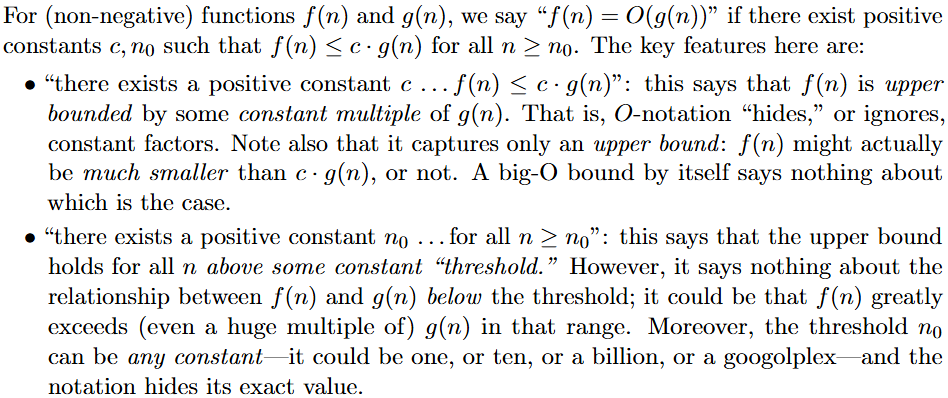
\includegraphics[width=\linewidth]{asymp.png}
      \end{center}
      \LaTeX\ you may need:
      \begin{itemize}
          \item In-line math
          \item Less-than-or-equal-to symbol
          \item Quote marks
          \item Lists
      \end{itemize}

      \begin{solution}
      % Uncomment this to include your solution
      % \begin{Verbatim}[breaklines]

      % \end{Verbatim}
      \end{solution}

    \part The following snippet is about \href{https://en.wikipedia.org/wiki/Fibonacci_sequence}{Fibonnaci numbers}. 
      \begin{center}
        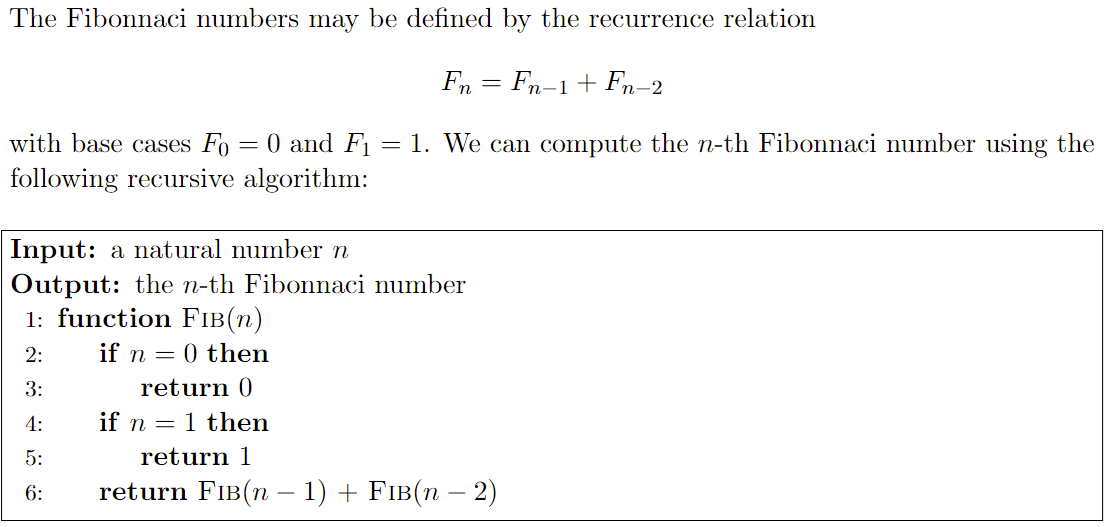
\includegraphics[width=\linewidth]{fib.png}
      \end{center}
    

    \LaTeX\ you may need:
    \begin{itemize}
        \item Display math
        \item The \texttt{algorithmic} environment
    \end{itemize}

    \emph{Hint:} Feel free to copy and modify the source code of the algorithms from other problems.

    \begin{solution}
      % Uncomment this to include your solution
      % \begin{Verbatim}[breaklines]

      % \end{Verbatim}
    \end{solution}

  \end{parts}

\ifprintanswers
\else
\newpage
\fi


  \question \textbf{Read the syllabus!}

  \begin{parts}

      \part [5]  Suppose you attend 9 out of 14 discussion sessions and submit both course evaluation receipts. Fill in the table below to calculate the weights of each component of your final grade. 
    \begin{center}
    \renewcommand{\arraystretch}{1.2}
    \begin{tabular}{|l|c|}
    \hline
    \textbf{Component}         & \textbf{Weight (\%)} \\ \hline
    Homework                   &  \\ \hline
    Exams                      &  \\ \hline
    Discussion Attendance      &  \\ \hline
    Course Evaluations         &  \\ \hline
    \textbf{Total}             & \textbf{100}       \\ \hline
    \end{tabular}
    \end{center}
      Based on your calculation, explain how attending 9 discussion impacts the weight distribution of your final grade compared to attending 10 or more discussions. 
      \begin{solution}
      Homework: 40\%, Exams: 59\%, Discussion Attendance: 0\%, Course Evals: 1\%. 

    Attending less than 10 discussions weights the final exam by an additional 3\%. 
      \end{solution}

      \part [5] Below is a table showing your scores for 12 homework assignments. Assume one homework was not submitted and one homework was submitted late. 

    \begin{center}
    \renewcommand{\arraystretch}{1.2}
    \begin{tabular}{|c|c|l|}
    \hline
    \textbf{Homework \#} & \textbf{Raw Score (\%)} & \textbf{Notes} \\ \hline
    1 & 100 & \\ \hline
    2 & 80 & \\ \hline
    3 & 90 & \\ \hline
    4 & 0 & Not submitted \\ \hline
    5 & 95 & \\ \hline
    6 & 70 & \\ \hline
    7 & 85 & \\ \hline
    8 & 88 & \\ \hline
    9 & 92 & \\ \hline
    10 & 50 & \\ \hline
    11 & 94 & \\ \hline
    12 & 90 & Submitted late\\ \hline
    \end{tabular}
    \end{center}

    Calculate your average homework grade after applying the drop policy (dropping the two lowest scores) and the 5\% late penalty.

    \begin{solution}

    \end{solution}

      \part [5] Name three different ways you can ask a question about course content in this class. How are you more likely to ask questions?

      \begin{solution}

      \end{solution}
  \end{parts}

\ifprintanswers
\else
\newpage
\fi

  \question \textbf{Welcome to EECS 376!}

  \emph{If you haven't already, please read \href{https://drive.google.com/file/d/1s8EuLp-75kDk3tE4_j18htpUnG4diVoq/view?usp=drive_link}{Handout 1} (Running Times and Aysmptotics) and apply it to the next three problems.}

To express our excitement for the start of EECS 376, we present an algorithm that prints \texttt{"Welcome to EECS 376!"} multiple times, based on two input parameters $n$ and $k$. You may assume that the \textsc{Print} operation runs in $O(1)$. 

\begin{minipage}{\linewidth}
\begin{algorithm}[H]
      \begin{algorithmic}[1]
        \Require{positive integers $n$ and $k \in \set{1,2, \ldots, n}$, both represented in base-2 (binary)}
        \Function{\text{Welcome}}{$n, k$} 
        \For{$i = 1, 2, \dots, k$}
            \For{$j = 1, 2, \dots, n-k$}            
            \State {\Call{Print}{\texttt{"Welcome to EECS 376!"}}}
            \EndFor
        \EndFor
        \EndFunction
      \end{algorithmic}
\end{algorithm}
\end{minipage}

\begin{parts}
    \part[3] Identify the value of $k$ that induces the \emph{most} \texttt{"Welcome to EECS 376!"} printed by the algorithm, in terms of $n$. \label{3a}
    \begin{solution}

    \end{solution}

    \part[4] Based on your answer in \cref{3a}, give the \emph{tightest correct asymptotic} (big-$O$) bound, as a function of~$n$, on the worst-case number of \texttt{"Welcome to EECS 376!"} printed by the algorithm. \label{3b}

    \begin{solution}

    \end{solution}

    \part[4] Determine whether the algorithm is \emph{efficient}, i.e., runs in at most polynomial time with respect to the input size. Briefly explain your answer. \label{3c}
    
    \emph{Reminder}: The input size of an integer is defined as the number of bits needed to represent it in binary.

    \begin{solution}

    \end{solution}

    \part [4] Does your answer in \cref{3c} change if $n$ and $k$ are represented in base-10 (decimals) instead? Briefly justify your answer.
    
    \emph{Hint:} You may want to use the change-of-base formula for logarithms for any positive real numbers $a$, $b$, and $c$, where $b \neq 1$ as well as $c \neq 1$: 
    \[
        \log_{b} a = \frac{\log_{c} a}{\log_{c} b}
    \]

    \begin{solution}

    \end{solution}
\end{parts}


    \question \textbf{Lumpy array.}
    
    In lecture, we said that you can measure the ``size" of an array as the number of elements in it, but we also said the ``size" of an input is the number of bits needed to represent it.  Consider the following example algorithm on an array:
       
    \begin{minipage}{\linewidth}
    \begin{algorithm}[H]
          \begin{algorithmic}[1]
            \Require{array $A$ of $n$ integers}
            \Ensure{sum of all elements in the array}
            \Function{\text{Sum}}{$A$}
            \State $S \gets 0$
            \For{$i = 1, 2, \dots, n$}
                \State $S \gets S + A[i]$
            \EndFor
            \State \Return $S$
            \EndFunction
          \end{algorithmic}
    \end{algorithm}
    \end{minipage}

\ifprintanswers
\else
\newpage
\fi

    \begin{parts}
        \part [5] For this part, we will assume that each element of the array is the same fixed size, and the ``size" of our input will be considered the number of elements in the array, $n$.  Find the big-O runtime of this algorithm (in terms of $n$) and state whether the function \textsc{Sum} is efficient, i.e., runs in polynomial time with respect to the input size ($n$). \label{4a}

        \emph{Note:} Because all elements of the array are the same size, we will treat addition as runnings in constant time, $O(1)$.

        \begin{solution}

        \end{solution}

        \part [5] Suppose instead, that we measure the ``size" of our array as the number of bits used to represent it, call it $b$.  Here, the elements of the array may be of different (arbitrarily large) sizes, so we will treat addition as running in linear time (to sum numbers with $k$ bits, it takes $O(k)$ time; you could think of this as taking finite time to add/carry each place value).  Determine whether in this interpretation, our algorithm is still efficient, running in polynomial time with respect to the input size (now $b$).
        
        \emph{Hint}: If our input has $b$ bits, find an upper bound on the number of elements that could be in the array and the number of bits in any one element of the array.  Note that your big-O bound for the runtime of the algorithm does not need to be a tight bound.

        \begin{solution}
            
        \end{solution}

    \end{parts}


  \question \textbf{Prof. Upsilon and their oopsie claims.}

  Prof. $\Upsilon$ is a brilliant but occasionally absent-minded computer scientist, known for their groundbreaking insights into algorithms—and the occasional ``oopsie" moments. Recently, $\Upsilon$ came up with three algorithms with the following running times:  
  
  \begin{itemize}
      \item Algorithm $X$ has running time $T_{X}(n) = O(n^2)$
      \item Algorithm $Y$ has running time $T_{Y}(n) = \Theta(n \log n)$
      \item Algorithm $Z$ has running time $T_{Z}(n) = \Theta(n)$
  \end{itemize}

  As usual, all running times are stated in terms of the \emph{worst case} for inputs of size~$n$.
  That is, $T_{X}(n)$ is the \emph{maximum} number of steps for which X runs, taken over all inputs of size~$n$ (and similarly for $T_{Y}, T_{Z}$).

  Now, Prof. $\Upsilon$ has made a series of claims about these algorithms.  State, with proof, whether $\Upsilon$'s claim is necessarily true, necessarily false, or not necessarily either based on the given information. If it is not necessarily either, give an example when it is true and an example when it is false. 

  \begin{parts}
    \part[6] ``We can upper bound the runtime of $Y$ by $O(n^2)$.''

    \begin{solution}
    
    \end{solution}

    \part[8] ``On every input, $Y$ runs faster than $X$.''
    \begin{solution}

    \end{solution}
    

    \part[10] ``For all large enough $n$, there is an input of size $n$ for which $Y$ runs faster than $X$.''
    \begin{solution}

    \end{solution}
    

    \part[10] ``For all large enough $n$, there is an input of size $n$ for which $Z$ runs faster than $Y$.''

    \begin{solution}

    \end{solution}

\end{parts}

    \question \textbf{Set of proofs by contra-.}
    
    Recall that a \emph{set} is a collection of distinct elements. Below are some important set notations:
    \begin{itemize}
        \item \textbf{Elements of a set:} $x \in A$ means $x$ os an element of set $A$. 
        \item \textbf{Complement of a set:} $\overline{A}$ \footnote{In some texts, you may encounter notations like $A^C$, $A^\complement$, $A'$, etc. to refer to the complement of $A$.} refers to the set of all elements in the universal set $U$ that are not in $A$.
        \item \textbf{Subset:} $A \subseteq B$ means every element of $A$ is also an element of $B$. 
        \item \textbf{Intersection of sets:} $A \cap B$ is the set of elements that are in both $A$ and $B$. 
        \item \textbf{Union of sets:} $A \cup B$ is the set of elements that are in $A$, in $B$, or in both.
        \item \textbf{Set difference:} $A \setminus B$ \footnote{Some texts may use $A - B$ to denote set difference.} is the set of elements that are in $A$ but not in $B$. We can also write it as $A \cap \overline{B}$.
    \end{itemize}

    \begin{parts}
        \part [5] Recall the transitive property of the subset relation: 
        \begin{quote}
            If $A \subseteq B$ and $B \subseteq C$, then $A \subseteq C$.
        \end{quote}
        Prove the above property by contradiction. 

        \begin{solution}

        \end{solution}

        \part [5] Recall the DeMorgan's Law, which says: 
        \begin{quote}
            If $x \in \overline{A \cap B}$, then  $x \in \overline{A} \cup \overline{B}$.
        \end{quote}
        State the contrapositive of the statement. Then, prove the contrapositive. 

        \begin{solution}

        \end{solution}
        
    \end{parts}

    
  \question \textbf{Euclid's algorithm, extended.}

  
  Given two integers $x,y$ (that are not both zero), one may wonder what values can be obtained by summing integer multiples of~$x$ and~$y$, i.e., expressed as $ax+by$ for some (not necessarily positive) integers $a,b$.
  It is not too hard to see that it is impossible to obtain any positive integer \emph{smaller} than their GCD $g = \gcd(x,y)$, because $ax+by$ must be divisible by~$g$.
  A less obvious fact is that the GCD \emph{can} be obtained in this way; this theorem is known as \emph{B\'{e}zout's identity} (pronounced ``BAY-zoo'').
    
  In this problem, you will modify the standard Euclidean algorithm to output not only $g=\gcd(x,y)$ itself, but also a pair $(a,b)$ of integers for which $ax+by = g$.
  (As we will see later, this is a very important tool for cryptography.)
  Such integers are called \emph{B\'{e}zout coefficients} for~$x,y$.
  We give most of the algorithm below:
    
    \begin{minipage}{\linewidth}
      \begin{algorithm}[H]
        \begin{algorithmic}[1]
            \Require{integers $x \geq y\geq 0$, not both zero}
            \Ensure{a triple $(g,a,b)$ of integers where $g = \gcd(x,y) = ax+by$}
            \Statex
            \Function{ExtendedEuclid}{$x,y$}
            \If{$y = 0$} \State \Return $(x,1,0)$
            \Comment{Base case: $1x + 0y = x = \gcd(x,0)$}
            \Else \State Divide $x$ by $y$, writing $x = qy + r$ for integer quotient $q$ and remainder $0\leq r < y$
            \State $(g,a',b') \gets \Call{ExtendedEuclid}{y,r}$
            \State [\textbf{FOR YOU TO DETERMINE:} compute appropriate $a$, $b$]
            \State \Return $(g, a, b)$
            \EndIf
            \EndFunction
        \end{algorithmic}
      \end{algorithm}
    \end{minipage}

  \begin{parts}
  
    \part[8] State what $a$ and $b$ should be on Line 7, and prove that the output is correct, i.e., that (1)~$g=\gcd(x,y)$, and (2)~$ax + by = g$.

    \emph{Hint}: by recursion/induction, we know that $g = \gcd(y,r)$ and $a'y+b'r = g$.
     
    \begin{solution}

    \end{solution}
    
    \part[8]
    Run the Extended Euclid algorithm by hand to find B\'{e}zout coefficients for the input $(x,y) = (376,281)$, and show that the output is correct.
    (You may use a calculator/computer only for the division steps.)
    Fill in the table below with a `trace' of the execution, i.e., all the variables' values in all the iterations.
    Also include the potential values $s = x+y$, the ratios (as fractions) of potentials $s_{i+1}/s_i$ for adjacent iterations, and Y/N indications of whether $s_{i+1}/s_i \leq 2/3$.

      \begin{table}[H]\centering
        \begin{tabular}{r|rr|rr|rr|rr|rrc}
          & \multicolumn{2}{c|}{input} & \multicolumn{2}{|c|}{division} & \multicolumn{2}{|c|}{rec ans} & \multicolumn{2}{|c|}{output} \\
          $i$ & $x$   & $y$  & $q$ & $r$  & $a'$ & $b'$ & $a$ & $b$ & $s$ & $s_{i+1}/s_{i}$ & $\leq 2/3$ ? \\ \hline
          $0$ & $376$ & $281$ &  &  &  &  &  &  &  &  &  \\
          % Add more rows as needed
        \end{tabular}
      \end{table}

    The entries labeled `input', `division', $s$, and $s_{i+1}/s_i$ should be filled from top to bottom, corresponding to the recursive calls; the `recursive answer' and `output' entries will need to be filled from bottom to top, corresponding to the `post-processing' (Line 7) of each recursive call's results.
    The entries for $a,b$ should match those of $a',b'$ one row above.
    Put~`--' for any entries that are not defined due to the base case.

    \begin{solution}

    \end{solution}
  \end{parts}




\end{questions}

\end{document}
